\section{Evaluation}\label{sec:evaluation}

In this section, we evaluate and compare the performance of our implementations of Fusionize, SAND, and ProFaaStinate.

\subsection{Fusionize and SAND}

%
% <TODO>
%

\paragraph{Experiment Setup}

for fusionize and sand we designed a benchmark aimed at isolating the network overhead to simulate cascading cold starts and double billing.
we chose method best showcases end to end latencies between FaaS functions. 
we decided for synthetic base load to investigate system's performance under maximum stress.
                                                                               
To showcase maximum latency, we designed two tasks, shown in Figure X, \emph{interface} task and \emph{counter} task. 
The counter Task receives a number and returns the number, incremented by one. 
The interface task receives a \emph{destination} number by the user and invokes the counter task, starting with the number zero. 
The result of the counter task is then used to invoke the counter task again until the destination number is reached.
                                                                               
This proposed load generator is unconventional, as it resides within the system under test. 
However, this design allows for function invocation within the platfrom and most importantly \emph{between} functions. 
To start the benchmark, only the interface task needs to be invoked with destination number and latency between invocation and result is to measured.

%
% </TODO>
%

\begin{figure}[!h]
    \centering
    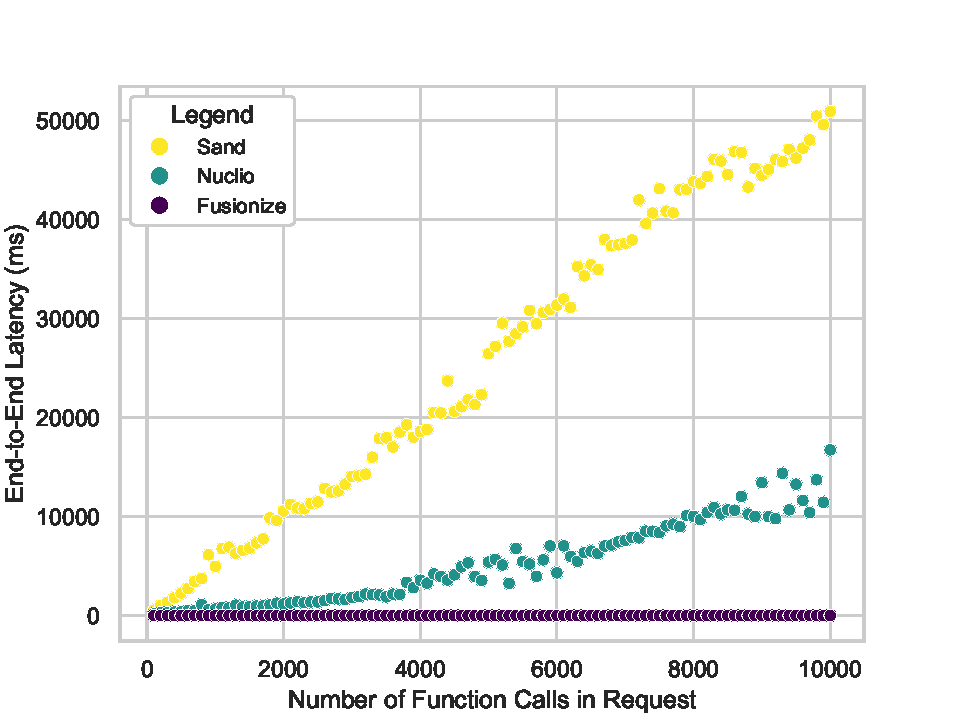
\includegraphics[width=\linewidth]{figures/latency_sand_fusionize.pdf}
    \caption{
        A comparison of end-to-end latency between our implementations of Fusionize, SAND, and vanilla Nuclio with increasing amounts of interaction between functions.
    }\label{fig:sand_fusionize}
\end{figure}

\paragraph{Results}

In figure~\ref{fig:sand_fusionize}, we can see the results of our benchmark. 
The x-axis shows the number of function calls required the answer the request, and the y-axis show the measured end-to-end latency.
As the interaction between functions increases, the end-to-end latency increases linearly for SAND. 
With 10,000 function calls, the SUT takes approximately 50 seconds to answer the request using our SAND implementation.
For vanilla Nuclio, the latency caused by the same request if significantly lower at below 20 seconds.
The end-to-end latency of vanilla Nuclio scales exponentially with increasing interaction between functions.
With Fusionize, the latency is very close to 0 throughout the experiment.

\paragraph{Interpretation of Results}

There are different possible explanations for the large differences between SAND, Fusionize, and vanilla Nuclio that we observed in our experiment.
To begin, all requests go through the Nuclio Dashboard using vanilla Nuclio.
In this case, the dashboard creates a large performance bottleneck, as all function calls have to pass through it.
Going through the dashboard for every request adds a lot of steps for the execution of the workflow: To invoke the next step, the request leaves its current function pod, enters a different pod—containing the Nuclio dashboard—only to be routed to another function pod again.
In comparison, the request does not leave its pod during the workflow using SAND. 
With SAND, a function call goes from a function processor to the local message bus, to a grain worker, to another function processor.
In our experiment, we observed better scalability but (significantly) worse performance with regard to latency.
An explanation for this is the environment the experiment was conducted in.
It is possible that the end-to-end latency using SAND would be lower than the latency using SAND while deploying Nuclio on a larger Kubernetes cluster, which would give SAND's components more resources, allowing it to improve its performance.
However, further experiments are required to confirm or deny this.
A difficulty for conducting experiments with Nuclio, in general, is its stability: Even with the load generated during our experiment, the Platform crashed multiple times, requiring multiple experiment runs to obtain the results.
This problem occurred more frequently as the number of function calls required to answer a request increased.
Lastly, the end-to-end latency of Fusionize appear near constant around 0 in figure~\ref{fig:sand_fusionize}.
While being slightly larger than zero and slightly increasing with more function calls, invoking the next workflow steps using Fusionize is done using local function calls. 
Comparing this to the relatively large networking overhead of both vanilla Nuclio and our SAND implementation reveals large differences in performance and scalability.

\subsection{ProFaaStinate}

%
% TODO
%

